\begin{figure}[htbp]
	\centering
	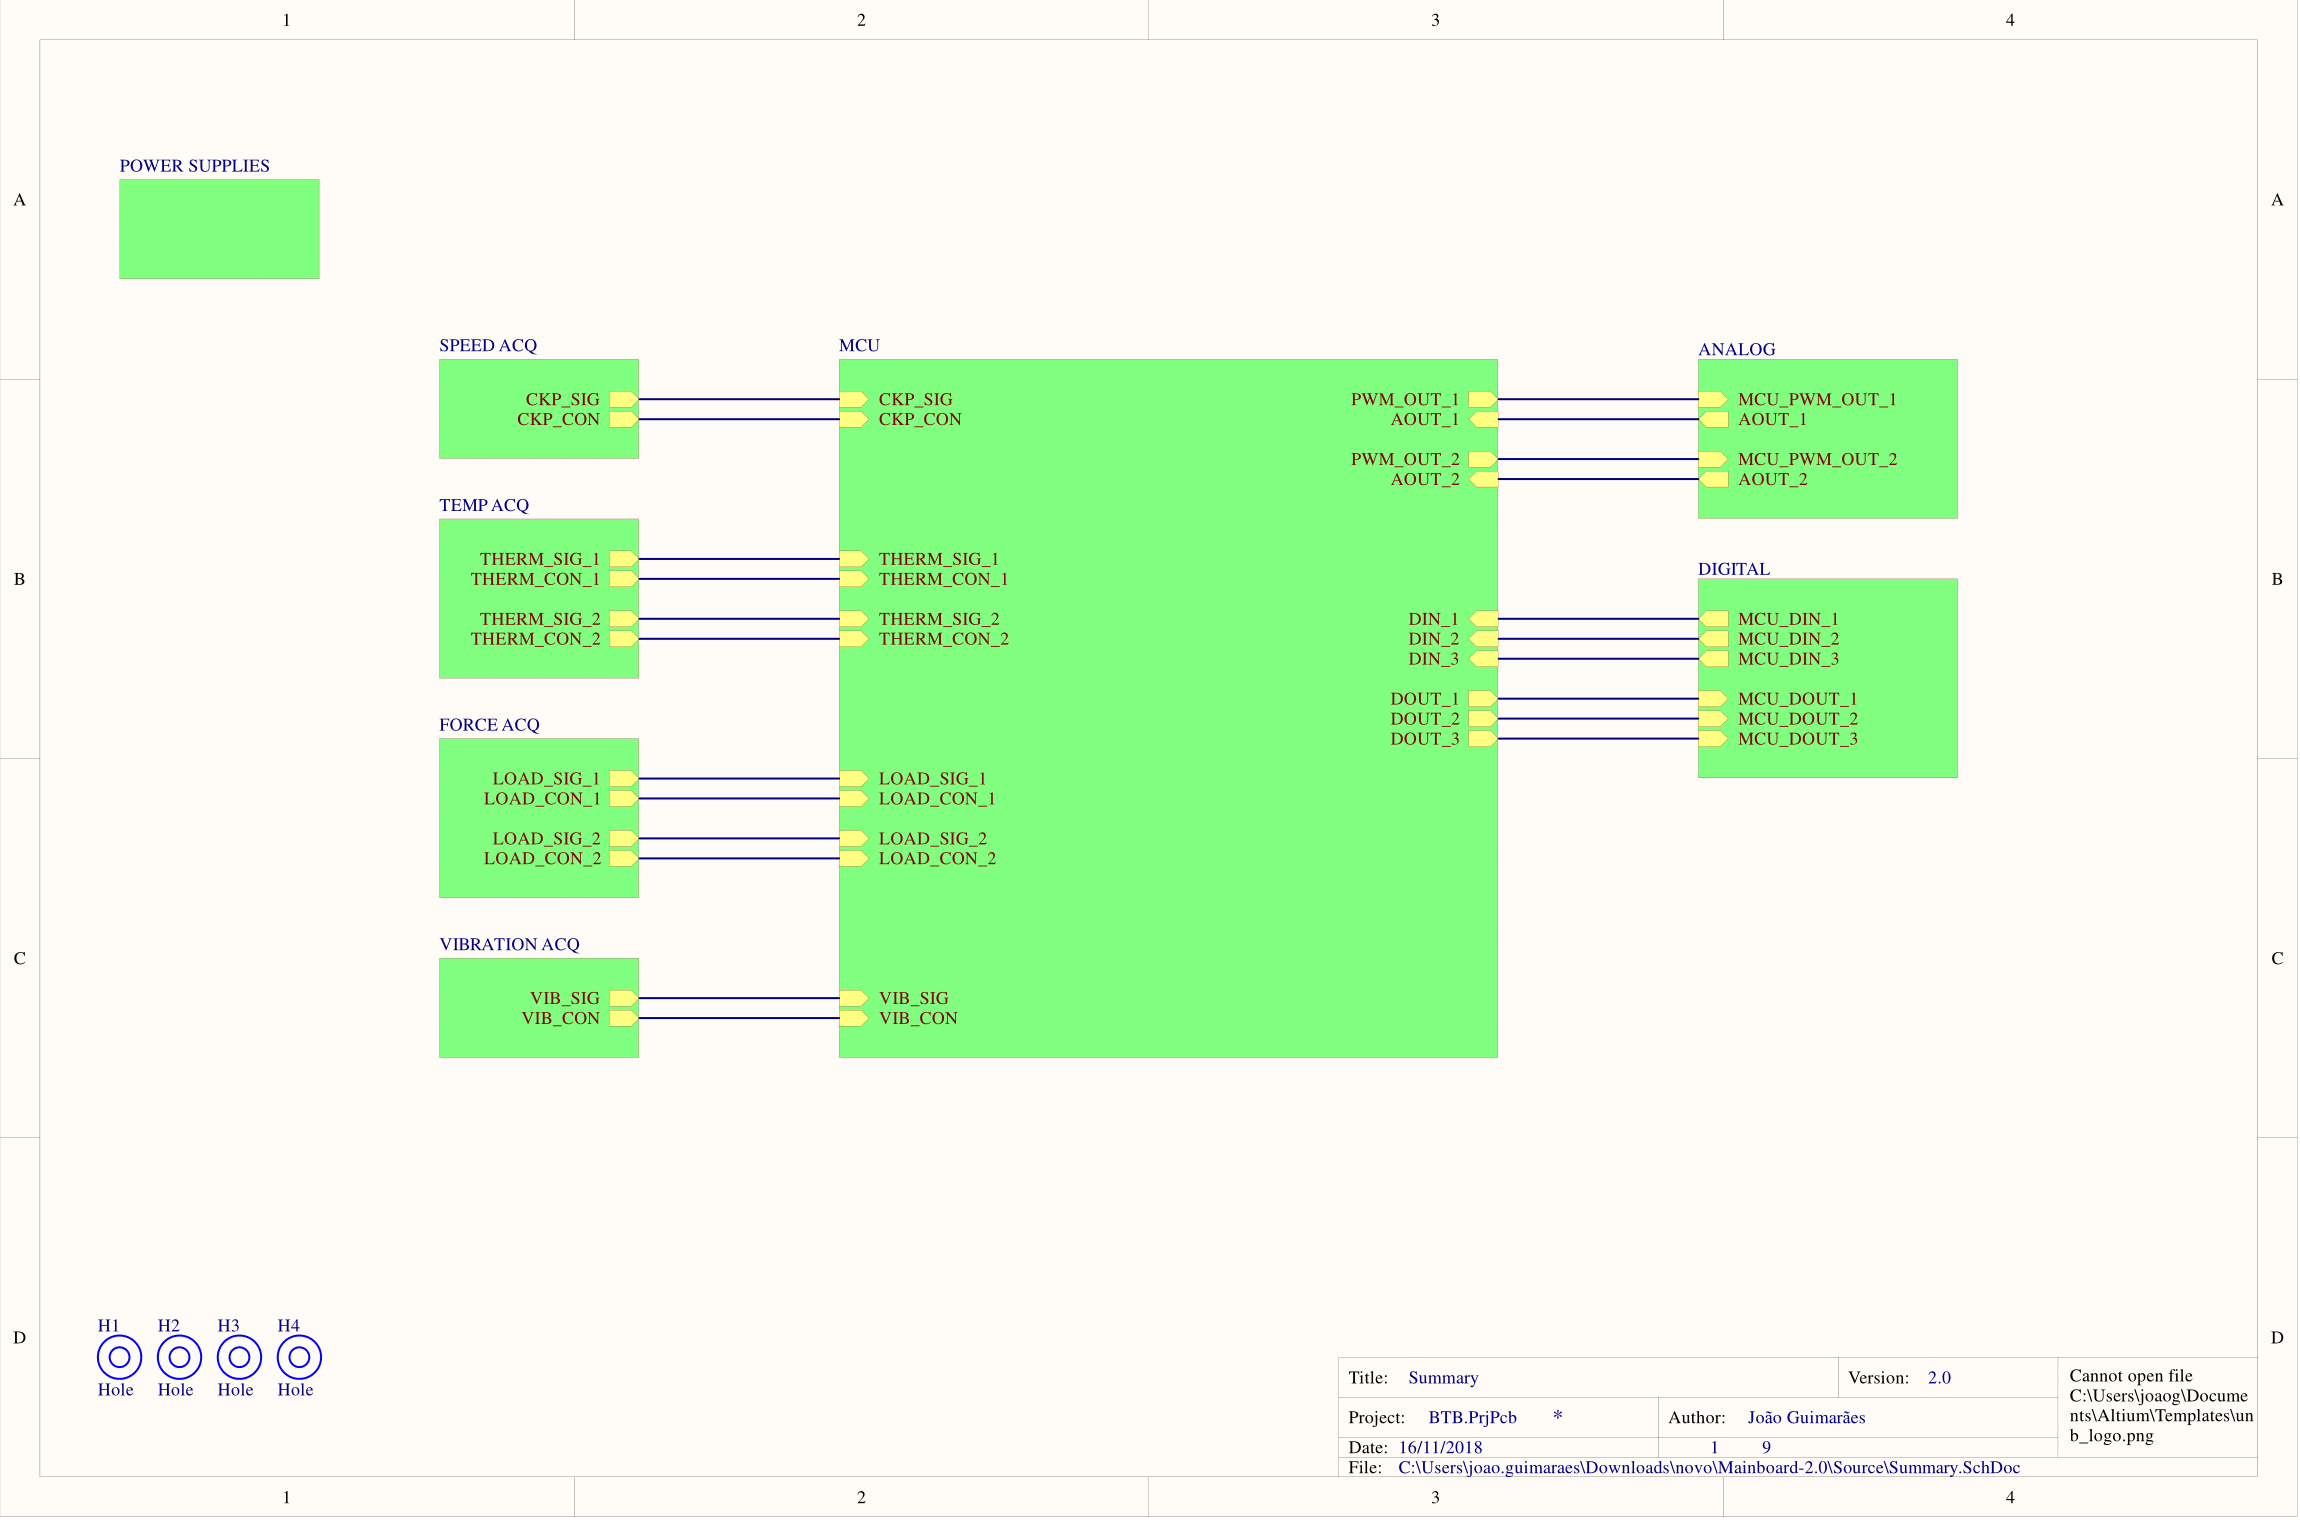
\includegraphics[width=1\textwidth, angle=270]{figuras/fig-schematic-1}
	%\caption{Frequency Inverter WEG-CFW08}
	%\label{fig:frequency-inverter}
\end{figure}

\begin{figure}[htbp]
	\centering
	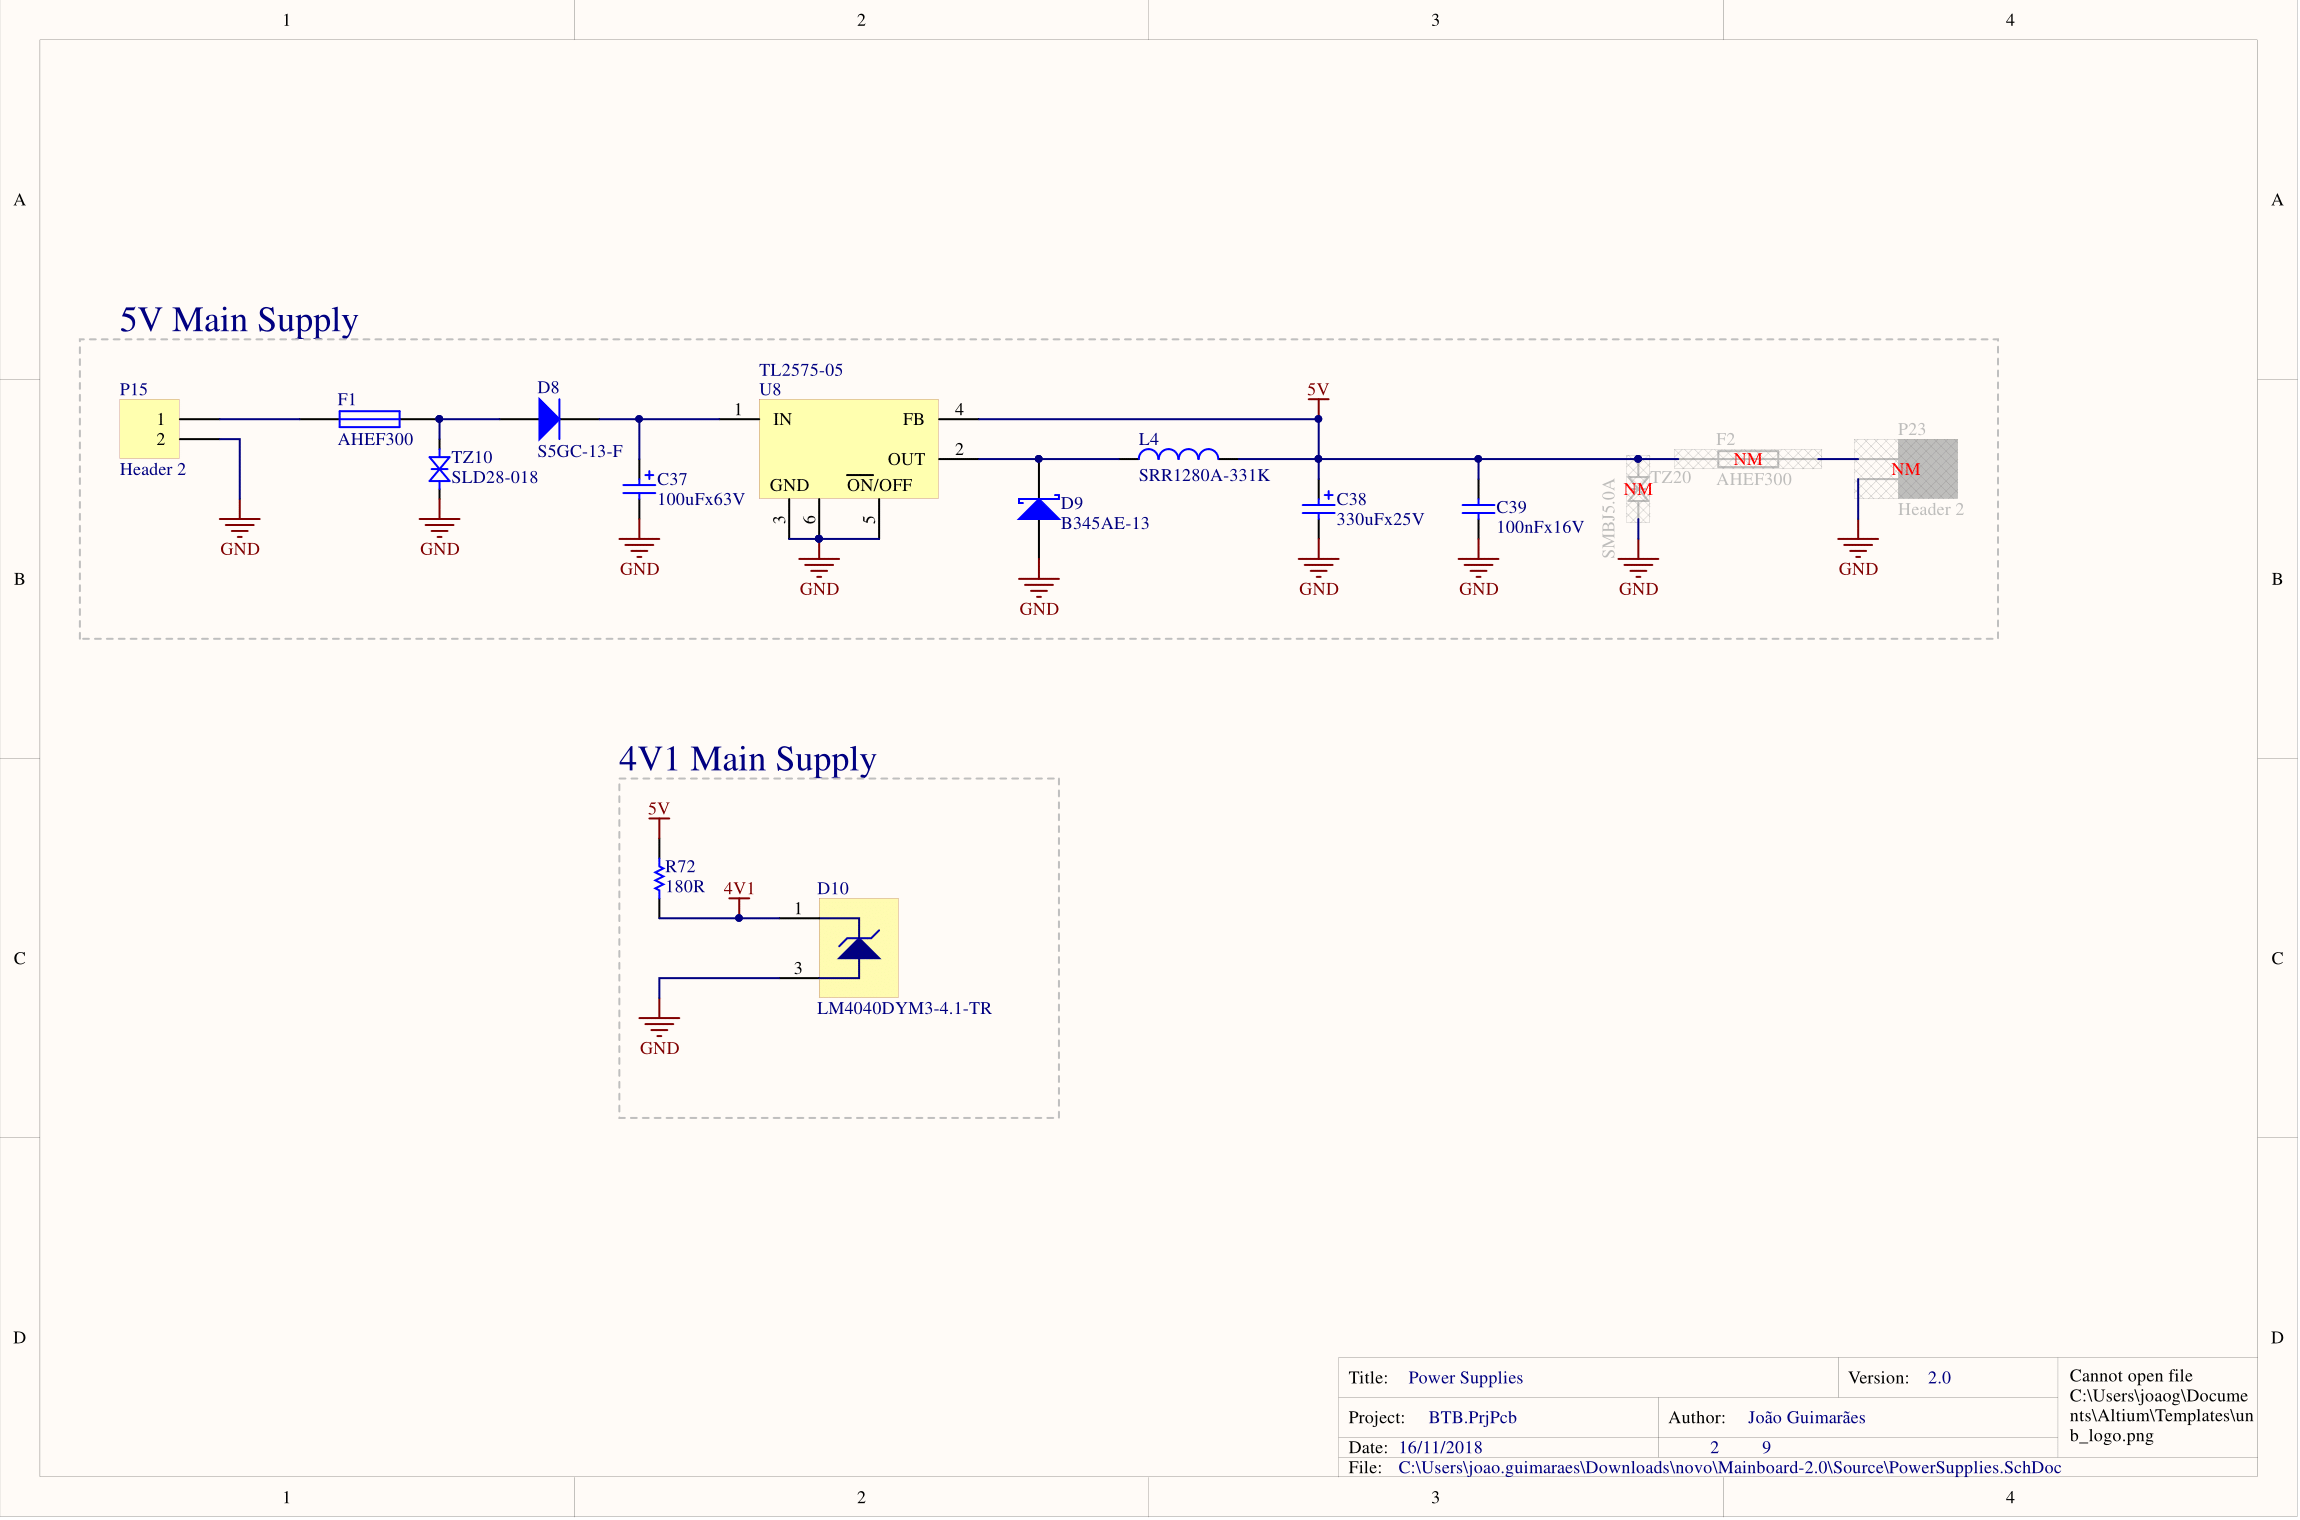
\includegraphics[width=1\textwidth, angle=270]{figuras/fig-schematic-2}
	%\caption{Frequency Inverter WEG-CFW08}
	%\label{fig:frequency-inverter}
\end{figure}

\begin{figure}[htbp]
	\centering
	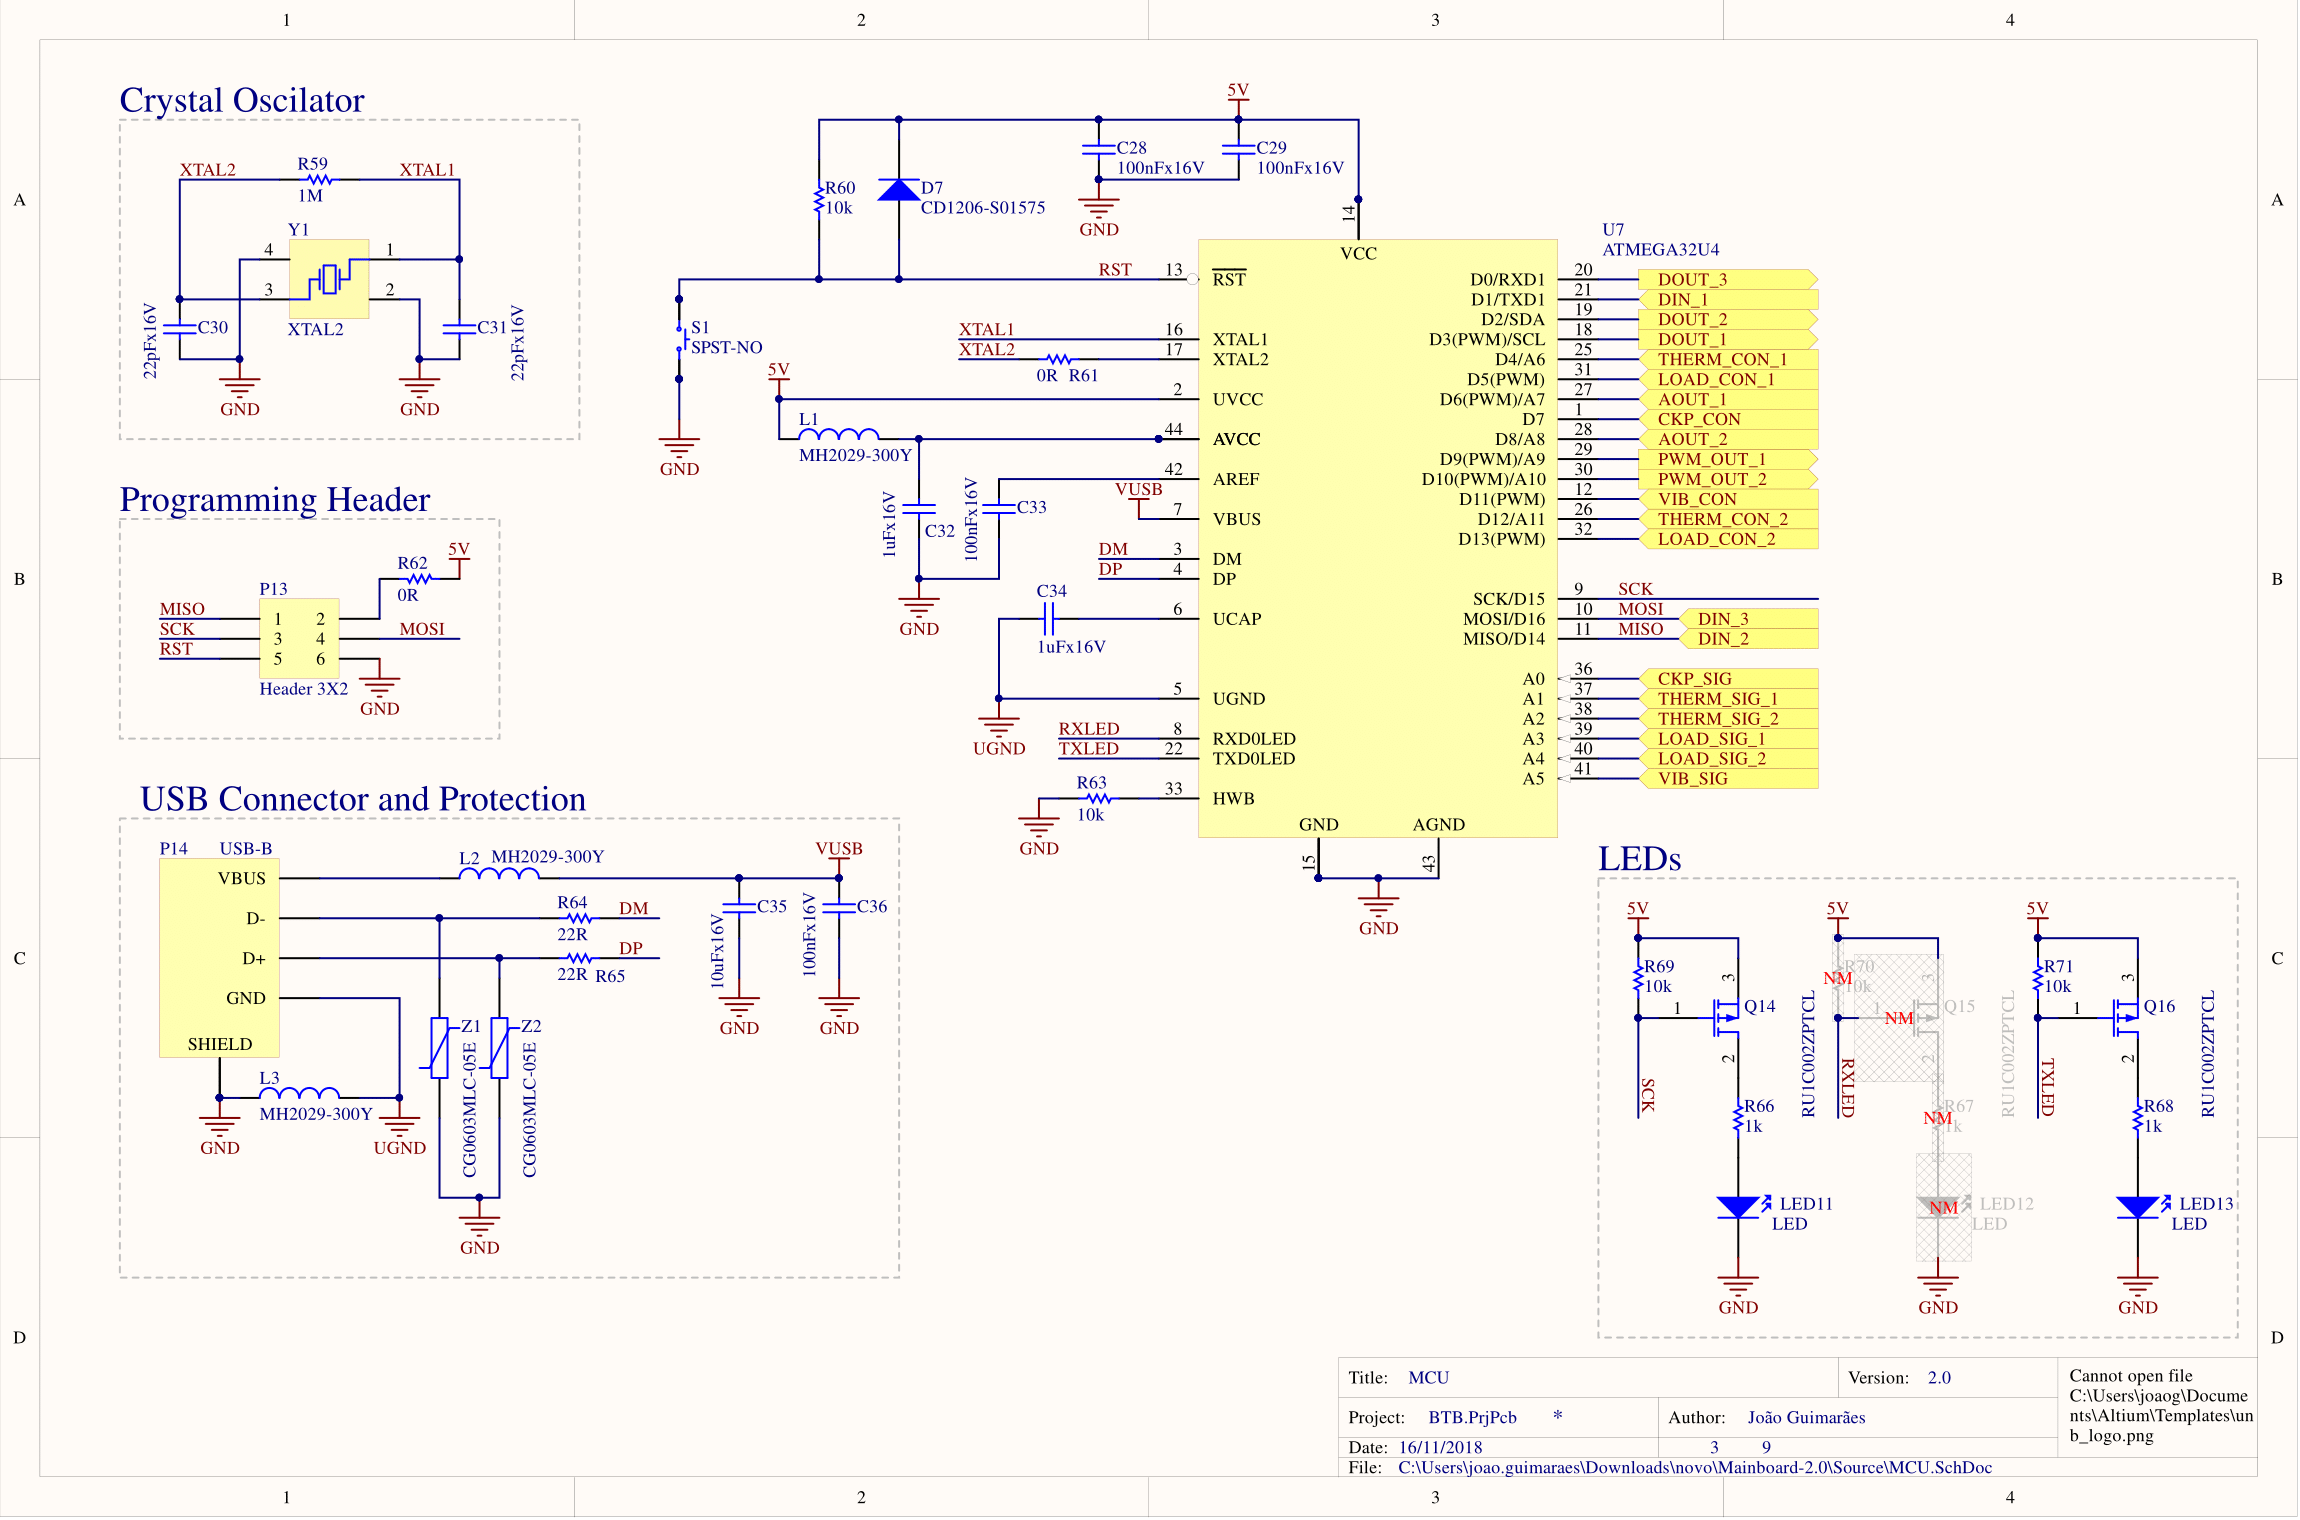
\includegraphics[width=1\textwidth, angle=270]{figuras/fig-schematic-3}
	%\caption{Frequency Inverter WEG-CFW08}
	%\label{fig:frequency-inverter}
\end{figure}

\begin{figure}[htbp]
	\centering
	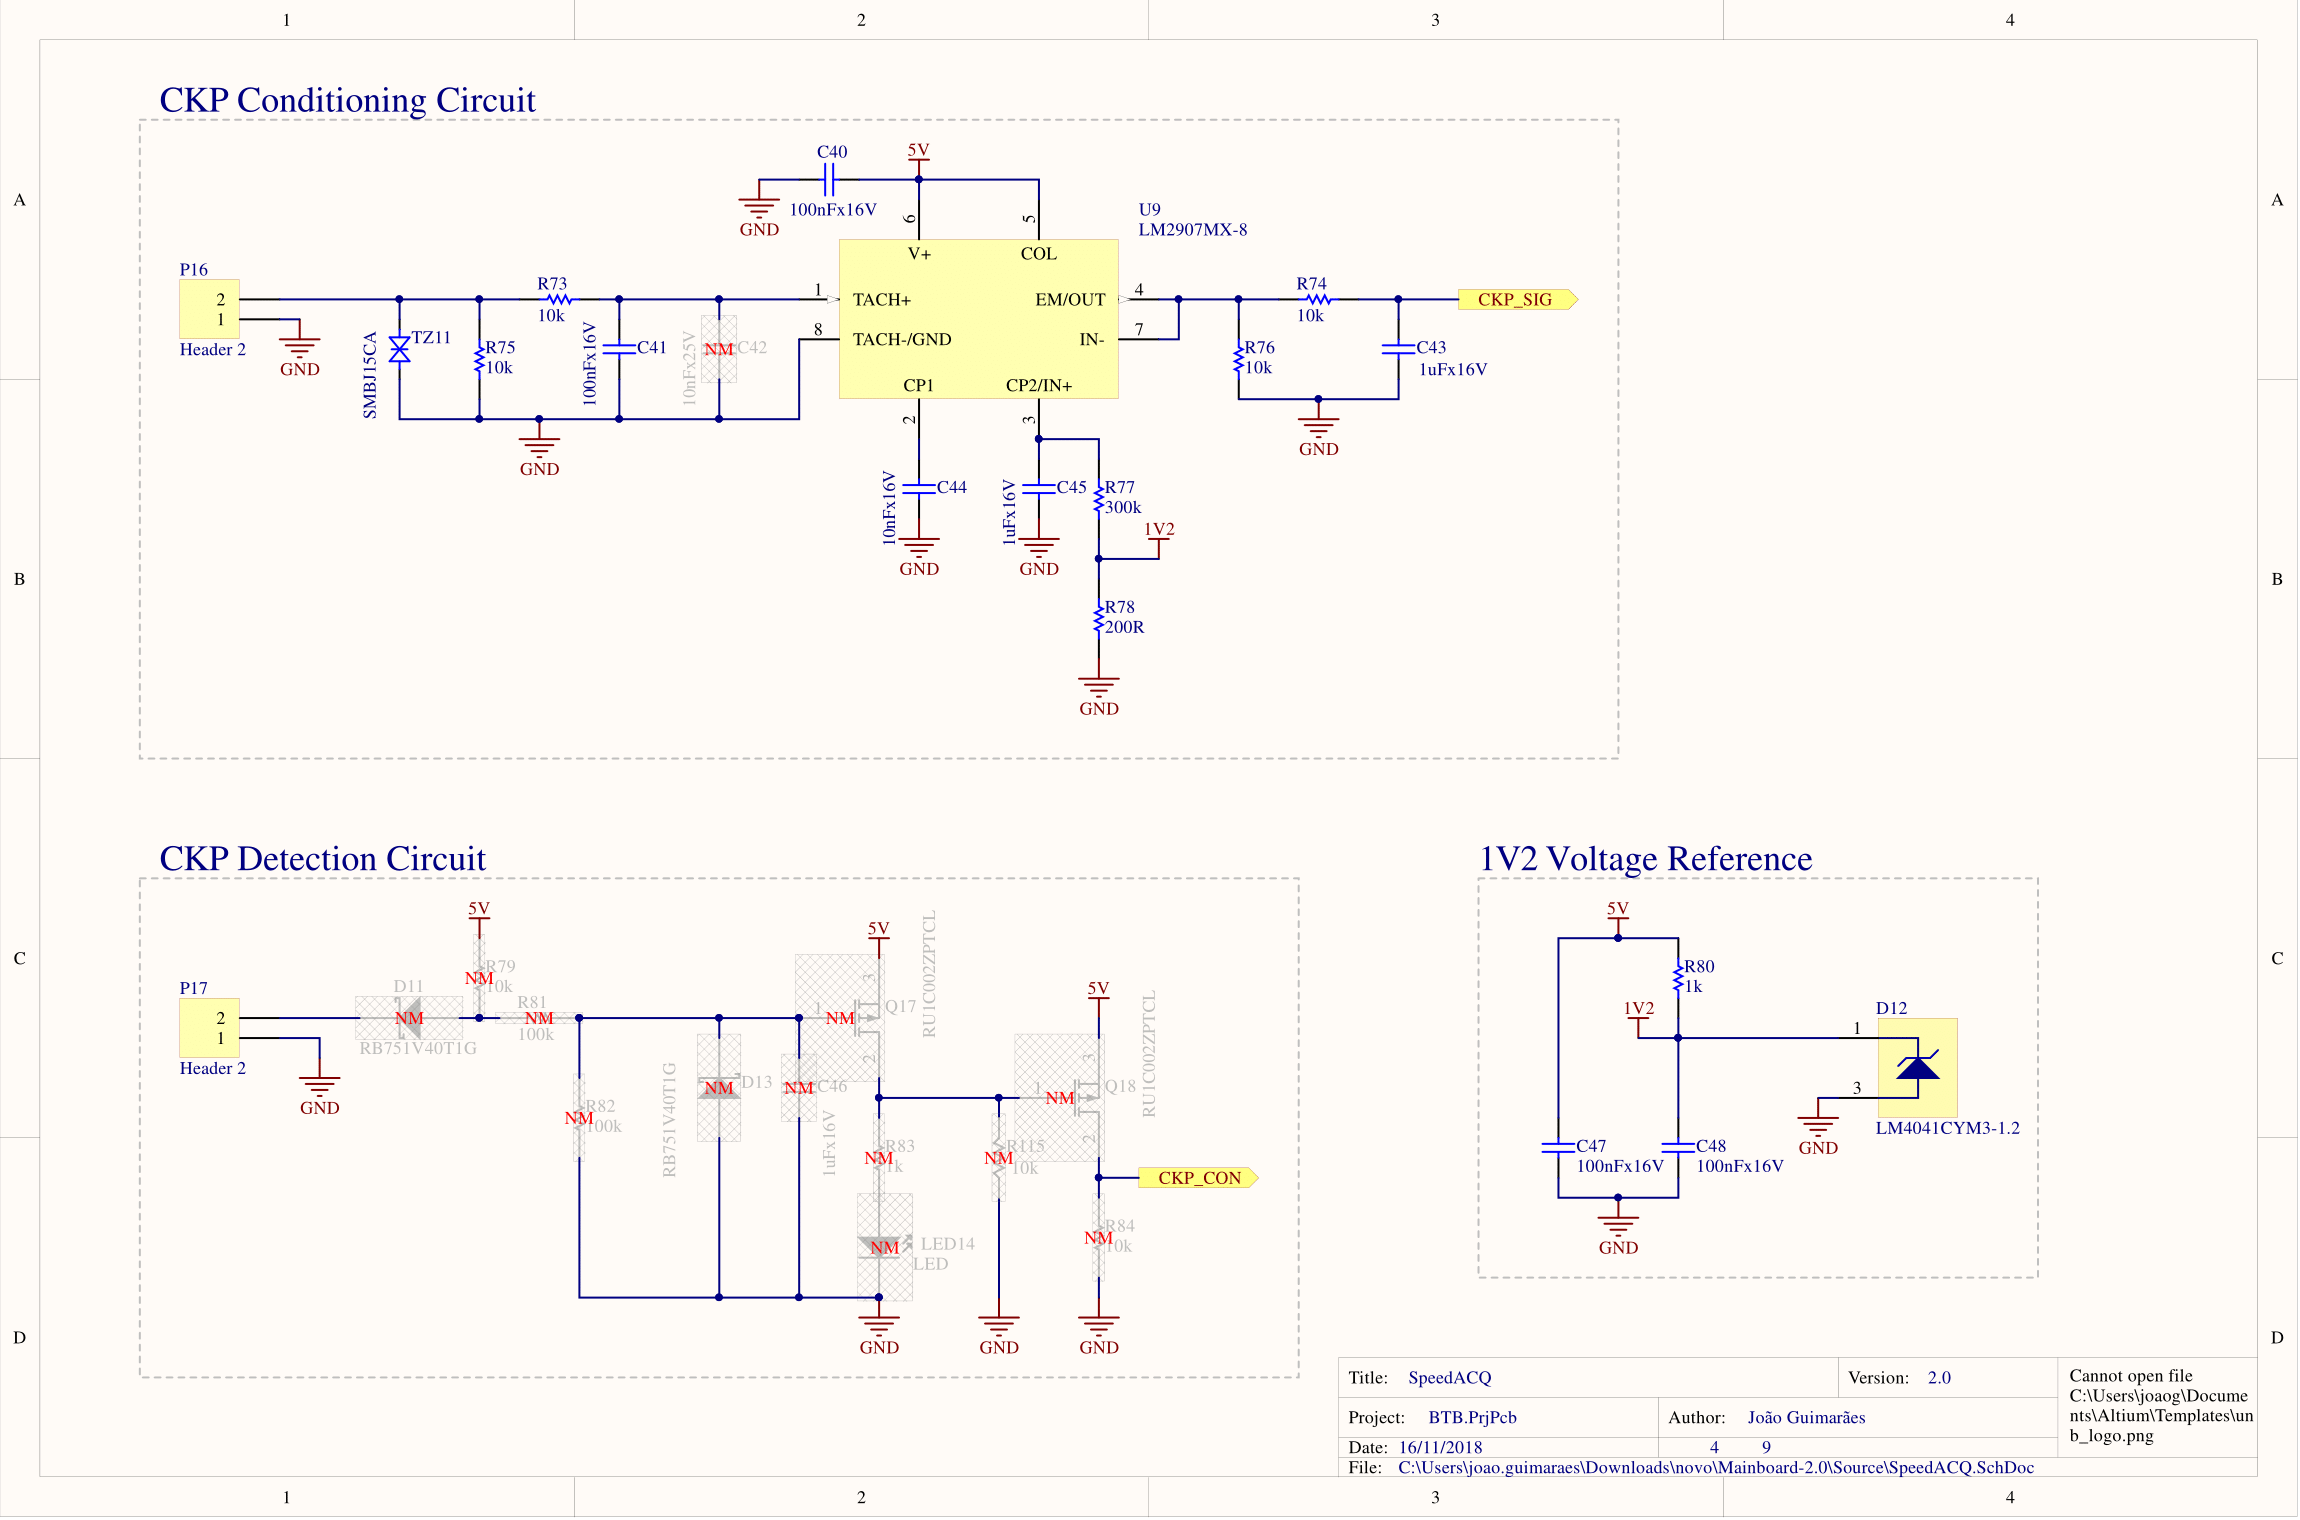
\includegraphics[width=1\textwidth, angle=270]{figuras/fig-schematic-4}
	%\caption{Frequency Inverter WEG-CFW08}
	%\label{fig:frequency-inverter}
\end{figure}

\begin{figure}[htbp]
	\centering
	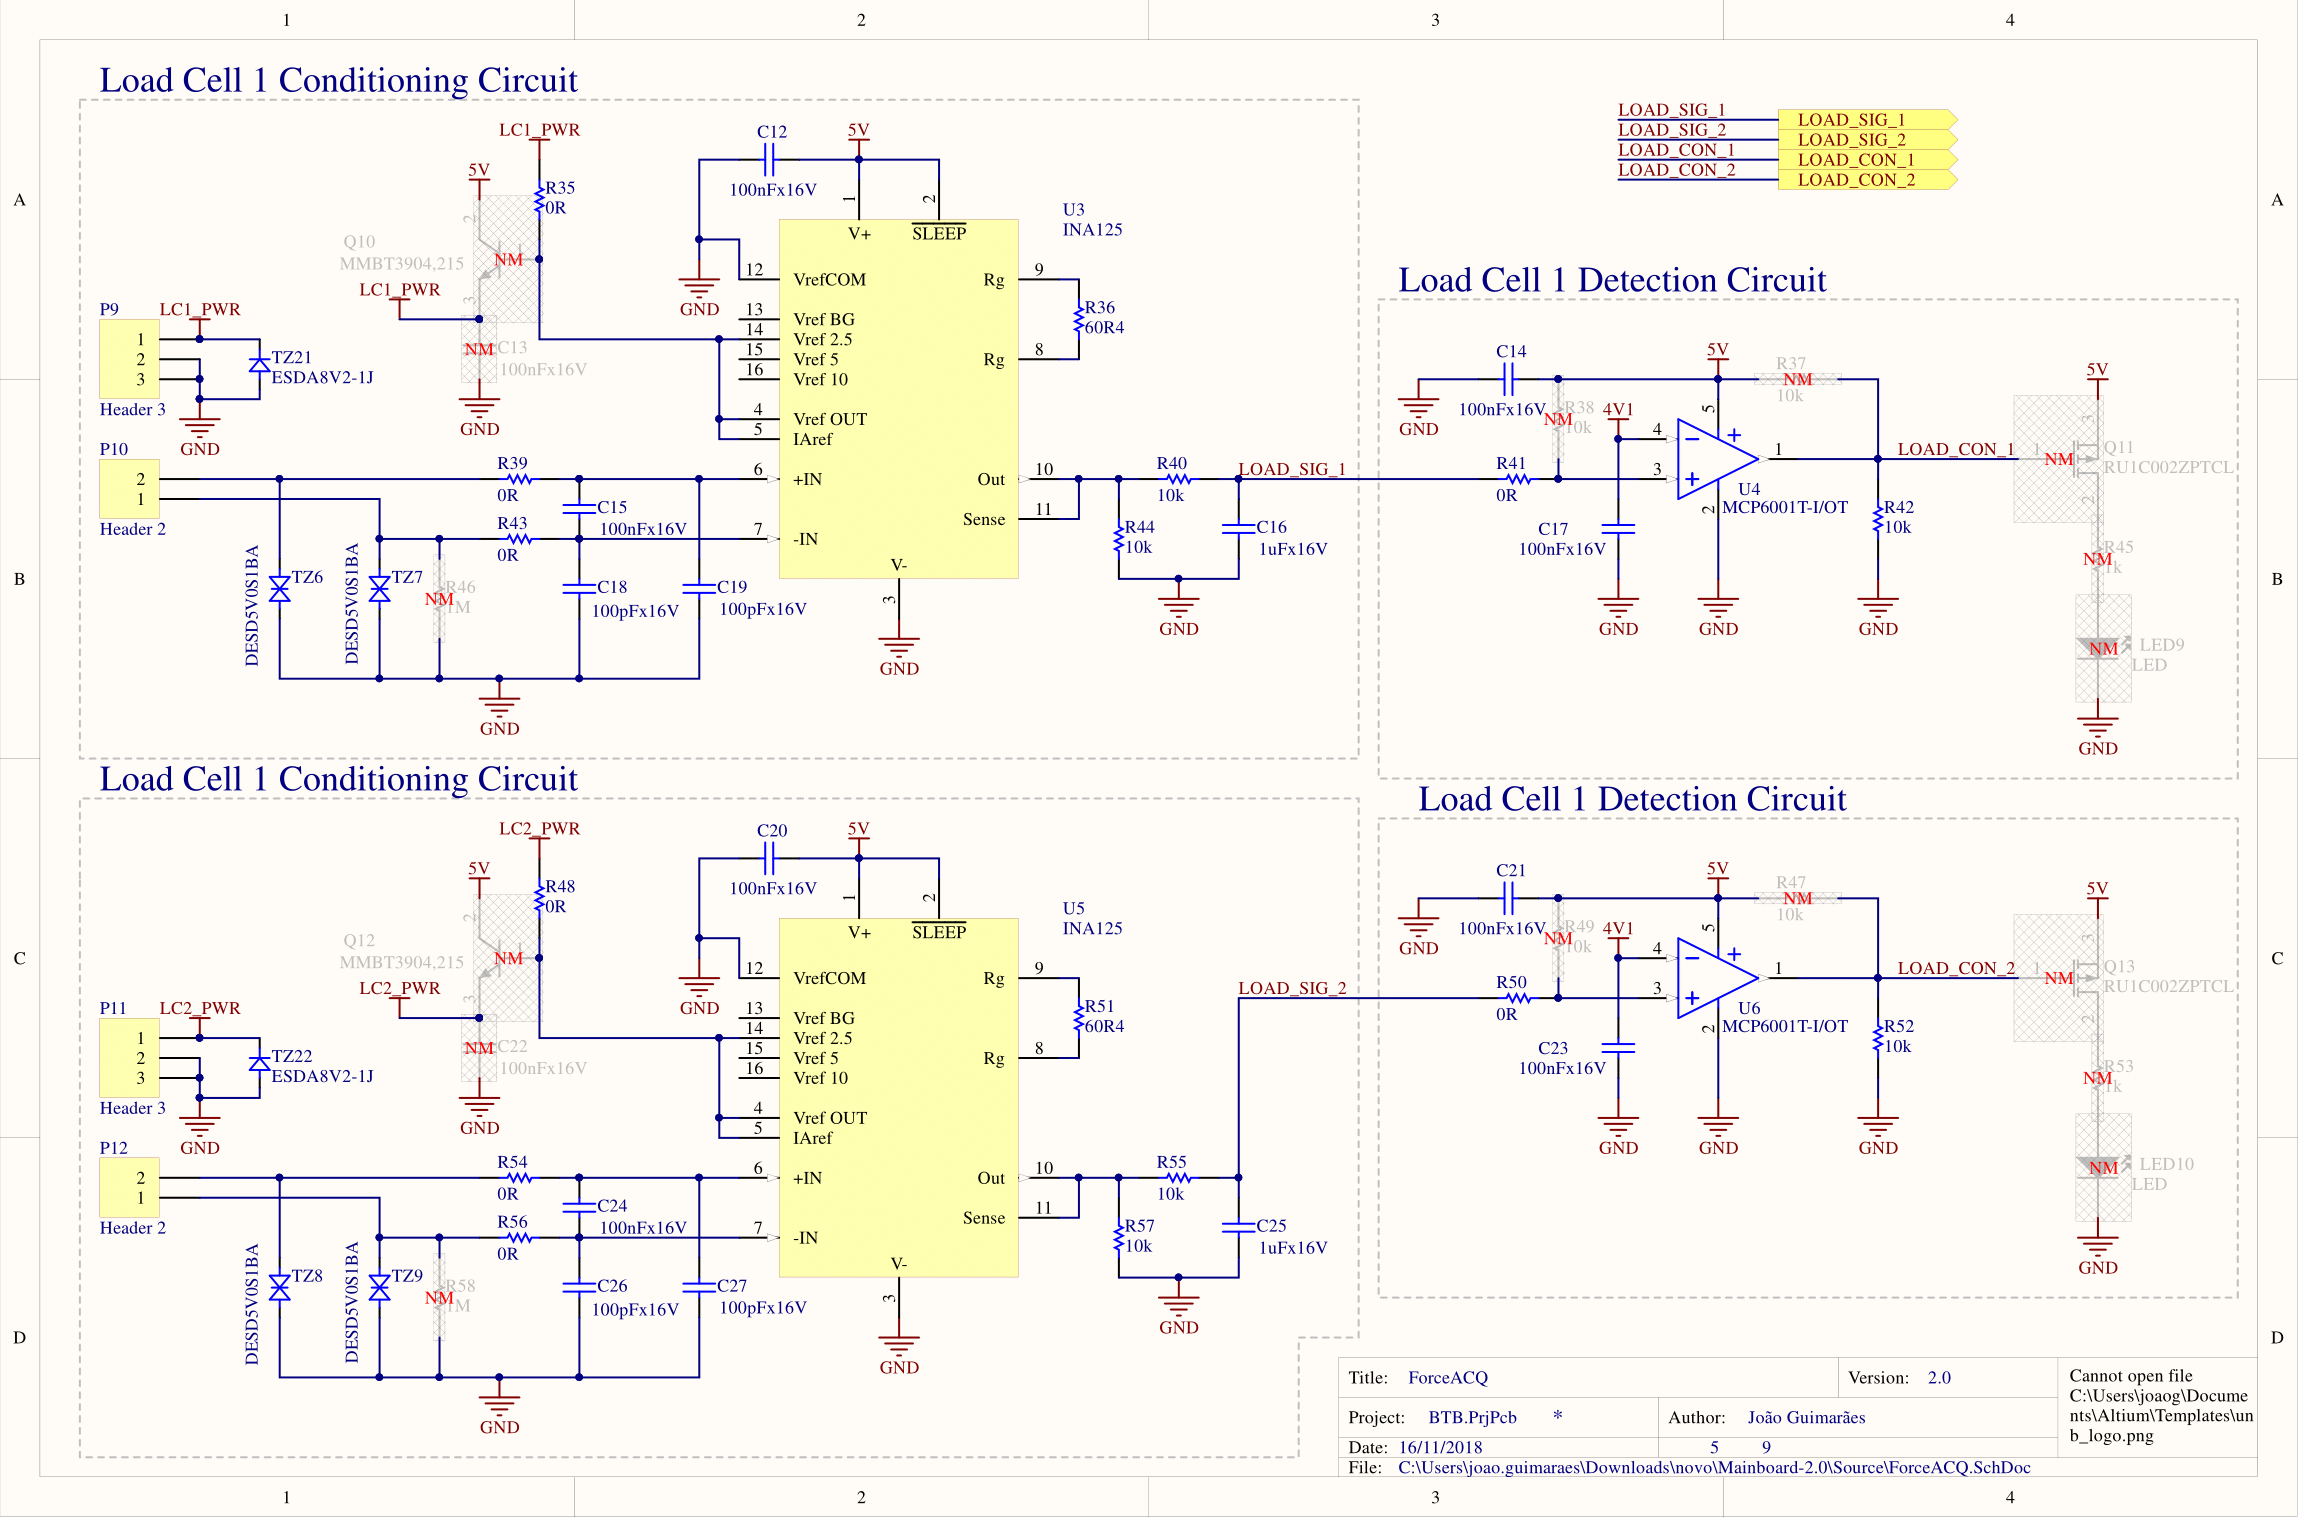
\includegraphics[width=1\textwidth, angle=270]{figuras/fig-schematic-5}
	%\caption{Frequency Inverter WEG-CFW08}
	%\label{fig:frequency-inverter}
\end{figure}

\begin{figure}[htbp]
	\centering
	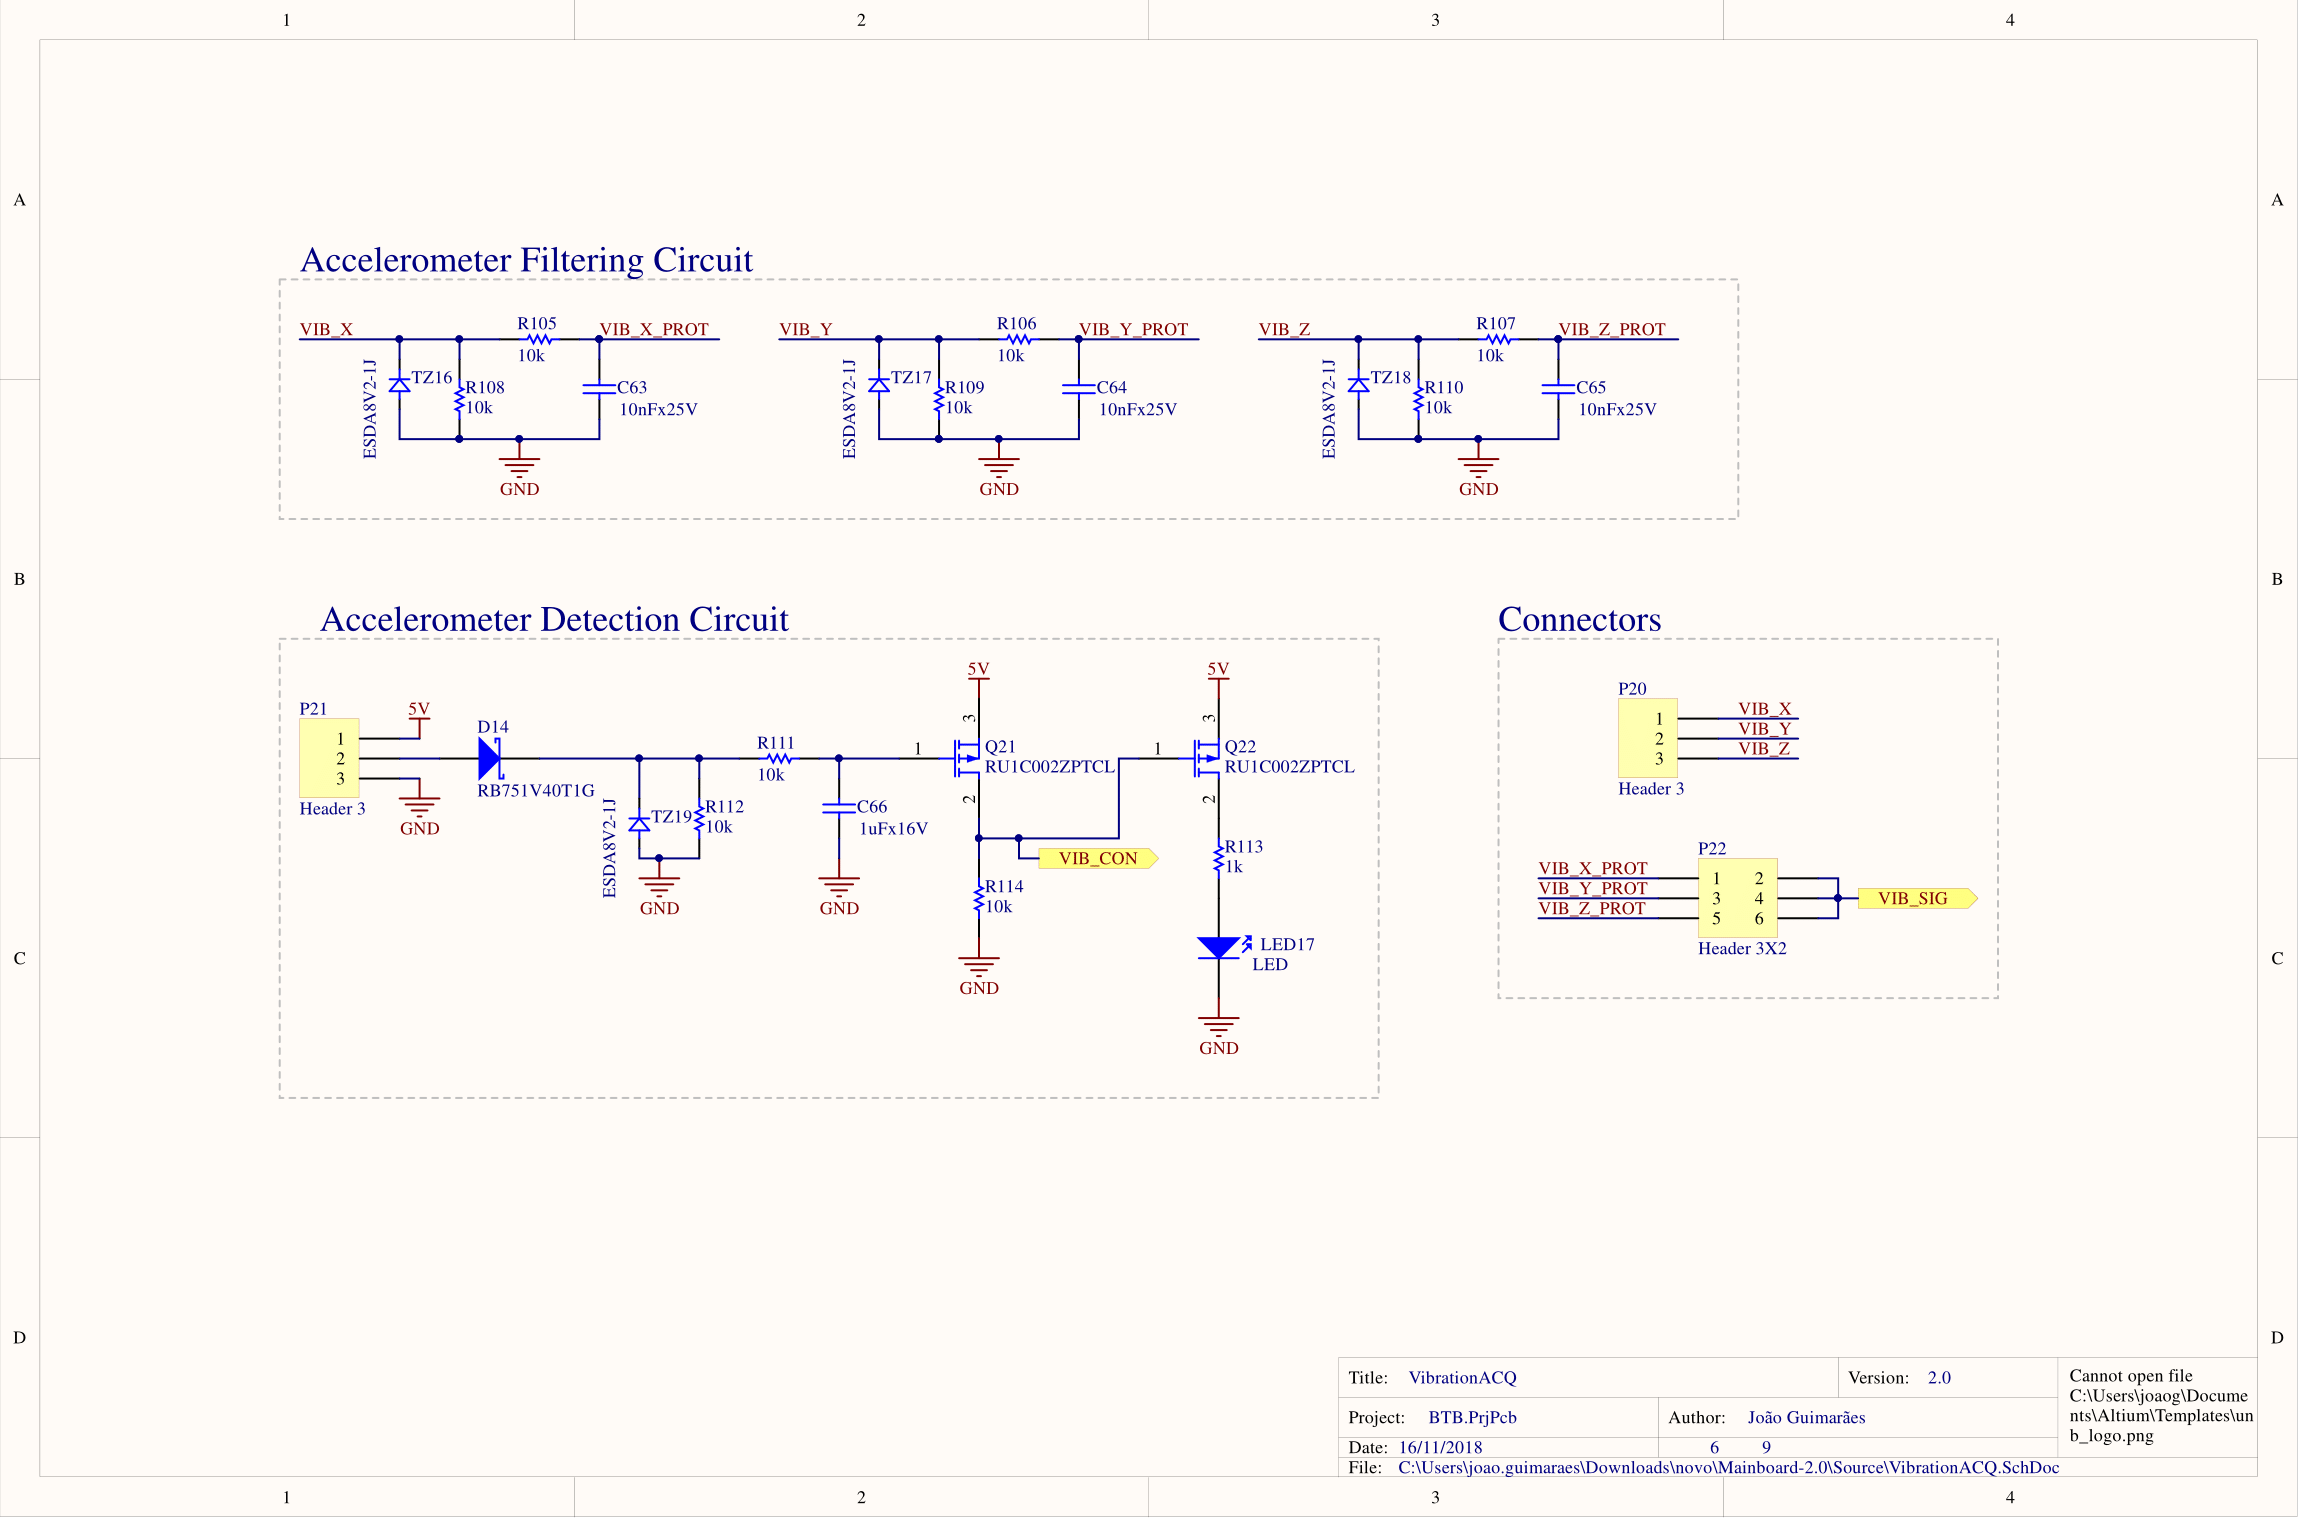
\includegraphics[width=1\textwidth, angle=270]{figuras/fig-schematic-6}
	%\caption{Frequency Inverter WEG-CFW08}
	%\label{fig:frequency-inverter}
\end{figure}

\begin{figure}[htbp]
	\centering
	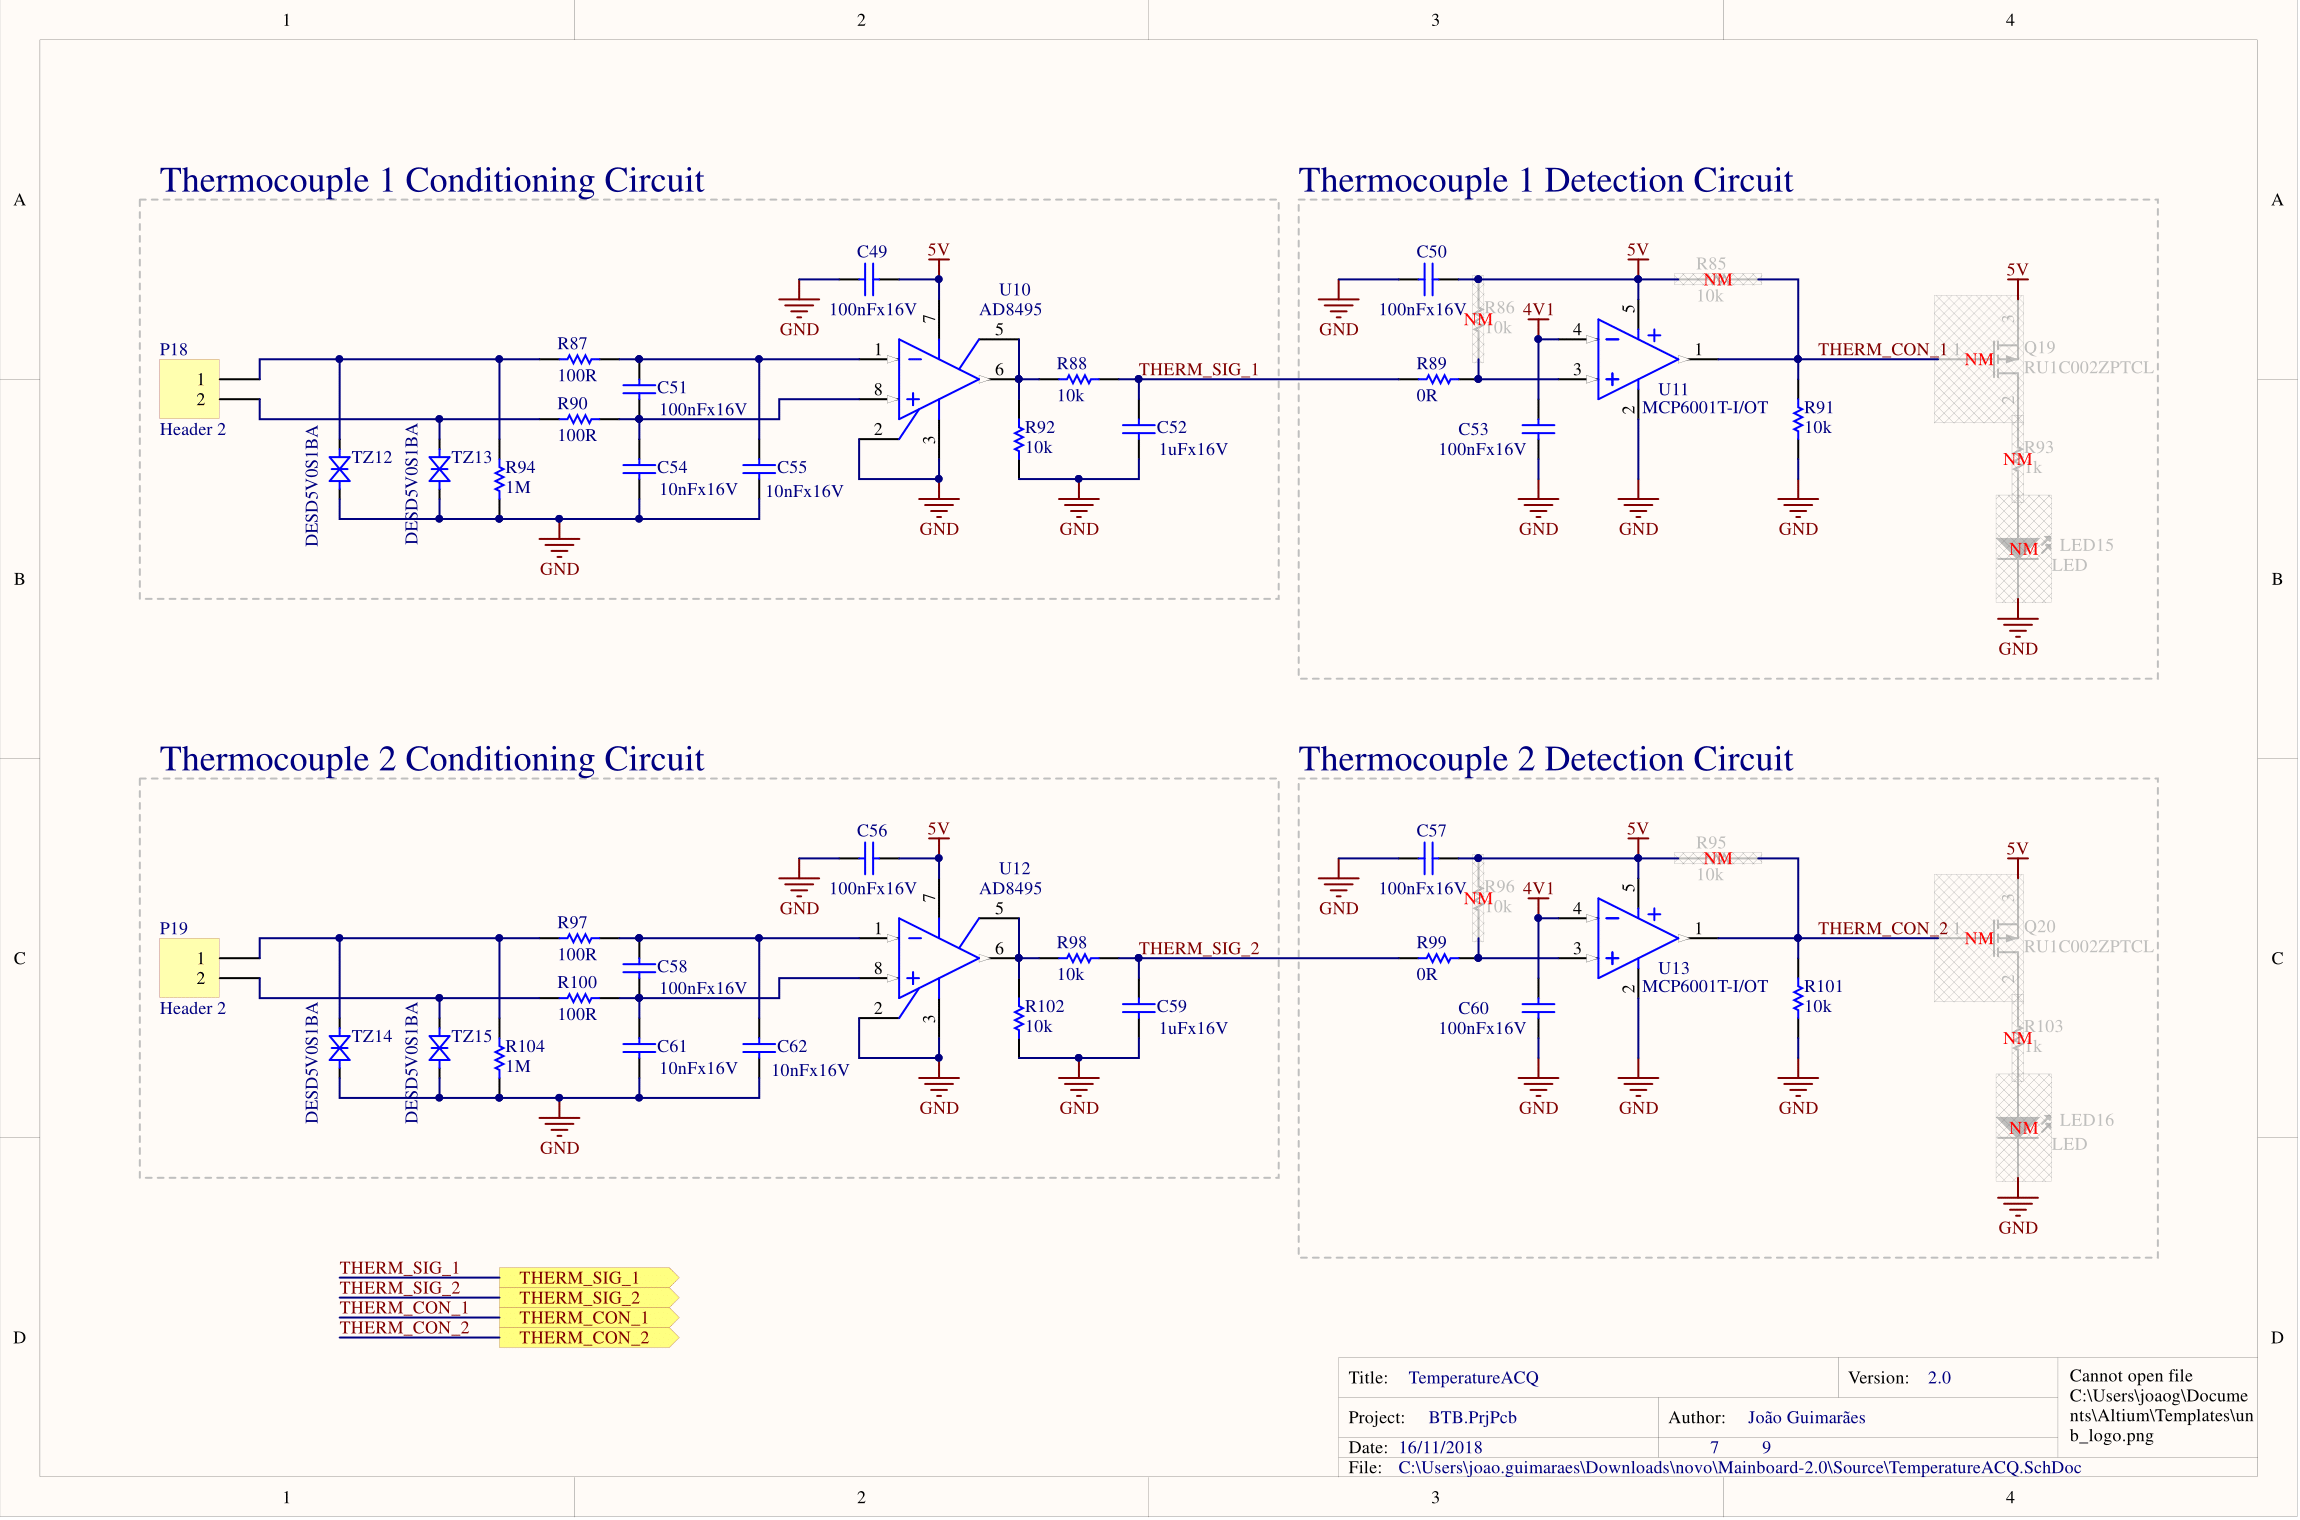
\includegraphics[width=1\textwidth, angle=270]{figuras/fig-schematic-7}
	%\caption{Frequency Inverter WEG-CFW08}
	%\label{fig:frequency-inverter}
\end{figure}

\begin{figure}[htbp]
	\centering
	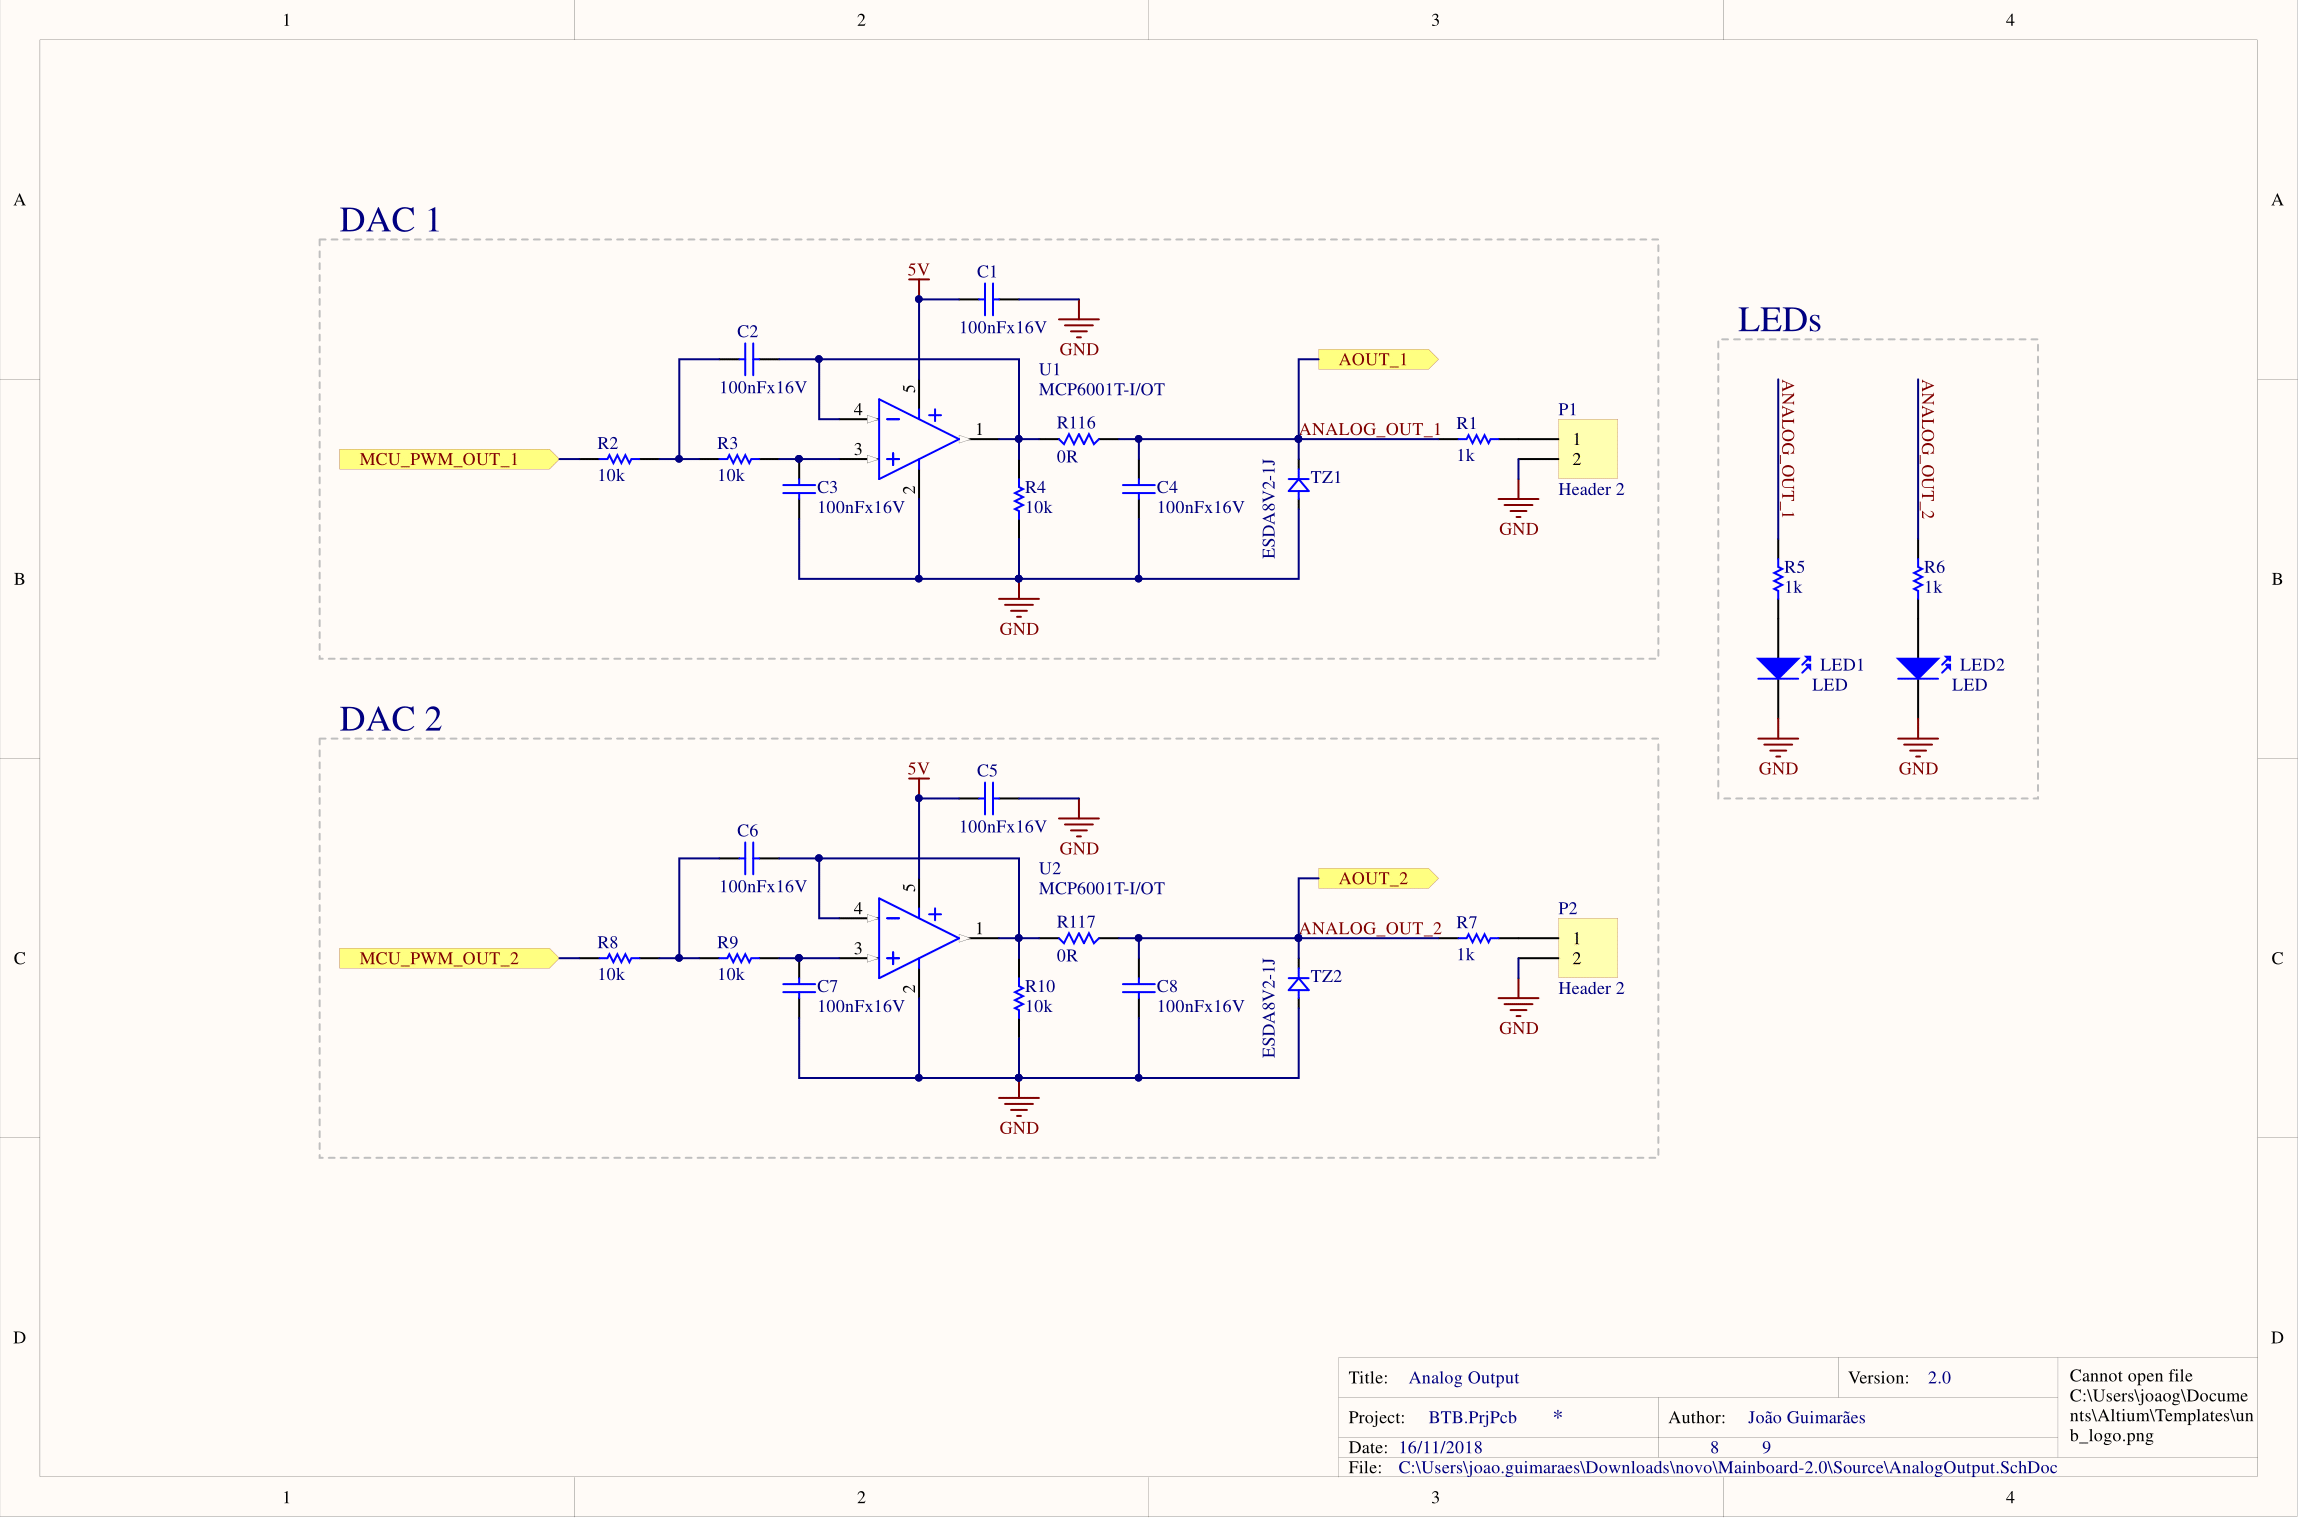
\includegraphics[width=1\textwidth, angle=270]{figuras/fig-schematic-8}
	%\caption{Frequency Inverter WEG-CFW08}
	%\label{fig:frequency-inverter}
\end{figure}

\begin{figure}[htbp]
	\centering
	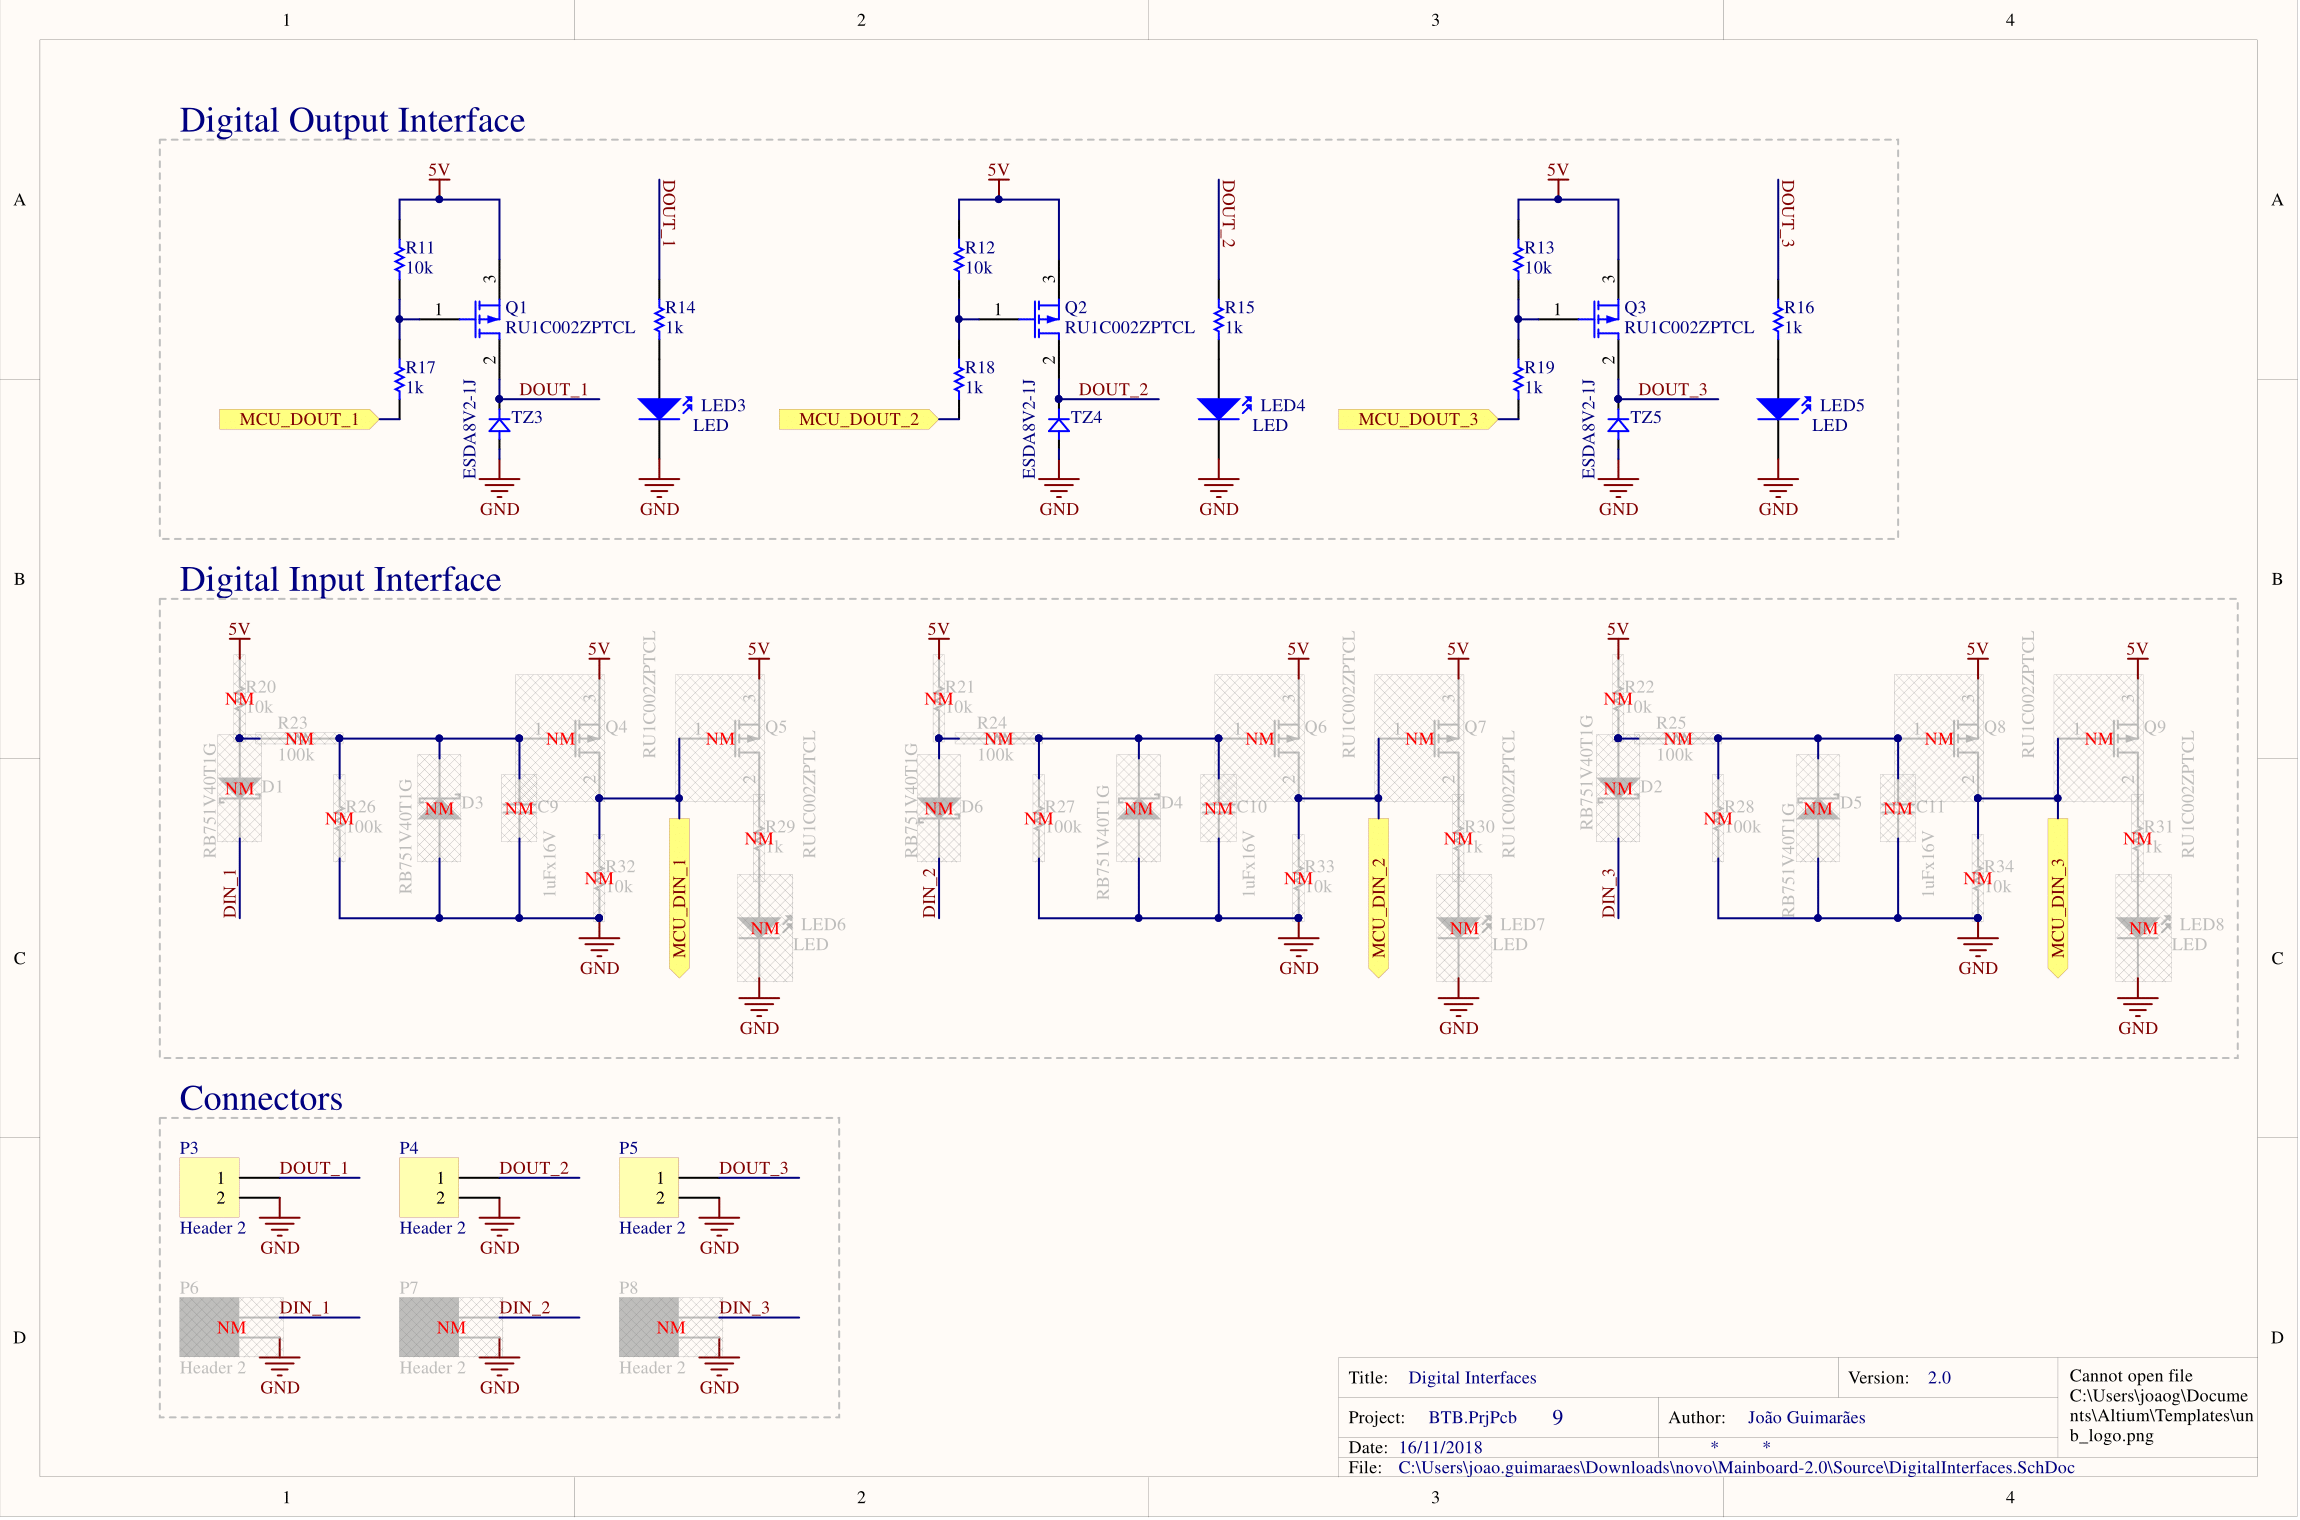
\includegraphics[width=1\textwidth, angle=270]{figuras/fig-schematic-9}
	%\caption{Frequency Inverter WEG-CFW08}
	%\label{fig:frequency-inverter}
\end{figure}